\documentclass[11pt,a4paper]{article}
\usepackage[margin=25mm]{geometry}
\usepackage{fontspec}
\setmainfont{TeX Gyre Pagella}
\setsansfont{TeX Gyre Heros}
\usepackage[french]{babel}
\usepackage{amsmath,amssymb,booktabs,tabularx,graphicx,float,placeins}
\usepackage{unicode-math}
\setmathfont{TeX Gyre Pagella Math}
\usepackage[authoryear,round]{natbib}
\usepackage{xcolor}
\usepackage{hyperref}
\usepackage{xurl}
\hypersetup{colorlinks=true,linkcolor=blue!45!black,citecolor=blue!45!black,urlcolor=blue!45!black,pdfauthor={Kun Huang}}
\usepackage{caption}
\captionsetup{font=small,labelfont=bf}
\setlength{\parskip}{4pt}
\setlength{\parindent}{14pt}
\setlength{\emergencystretch}{2em}
\renewcommand{\arraystretch}{1.15}
\newcommand{\notes}[1]{\par\vspace{3pt}{\footnotesize\noindent\textit{Note :} #1\par}}
\newcommand{\source}[2]{\href{#1}{#2}}
\newcommand{\BorderCoef}{0,146}
\newcommand{\BorderLo}{0,051}
\newcommand{\BorderHi}{0,241}
\newcommand{\BorderSE}{0,048}
\newcommand{\BroadCoef}{-0,007}
\newcommand{\BroadLo}{-0,065}
\newcommand{\BroadHi}{0,052}
\newcommand{\MatchedCoef}{-0,017}
\newcommand{\MatchedLo}{-0,100}
\newcommand{\MatchedHi}{0,066}
\newcommand{\BorderPairs}{774}
\newcommand{\NewN}{2\,117}
\newcommand{\ControlN}{14\,361}
\newcommand{\MatchedPairs}{1\,908}
\newcommand{\PanelN}{3\,068\,820}
\newcommand{\CommuneN}{34\,098}
\newcommand{\BirthN}{11\,285\,045}
\newcommand{\ULBirthN}{6\,953\,847}
\newcommand{\ShortPreP}{0,489}
\newcommand{\SeasonPreP}{0,000157}
\newcommand{\AnnualPreP}{0,238}
\newcommand{\PPMLRatio}{1,056}
\newcommand{\MapFRRN}{17\,622}
\newcommand{\PPMLPairs}{757}
\newcommand{\PPMLExcluded}{17}
\newcommand{\WildP}{0,0077}
\newcommand{\FRRInitialN}{17\,717}
\newcommand{\FRRInitialPartialN}{20}
\newcommand{\OldZRRFullN}{17\,694}
\newcommand{\OldZRRPartialN}{36}
\newcommand{\FRRAdditionsAprN}{117}
\newcommand{\FRRCoreJulyN}{17\,789}
\newcommand{\FRRCorePartialJulyN}{20}
\newcommand{\FRRBenefJulyN}{2\,145}
\newcommand{\FRRBenefPartialJulyN}{11}
\newcommand{\FRRPlusJulyN}{4\,456}
\newcommand{\StableNeverN}{14\,611}
\newcommand{\StableLaterCoreExcludedN}{116}
\newcommand{\BorderCommuneN}{1\,548}
\newcommand{\EPCIComponentsN}{128}
\newcommand{\EDComponentsN}{46}
\newcommand{\EDBComponentsN}{36}
\newcommand{\EDBMaxPairsN}{191}
\newcommand{\HQBirthN}{10\,175\,417}
\newcommand{\NonHQBirthN}{1\,101\,326}
\newcommand{\UnknownHQN}{8\,302}
\newcommand{\UnknownAgeN}{29\,742}
\newcommand{\AgeFlaggedN}{24}
\newcommand{\AssignmentMetroN}{34\,816}
\newcommand{\AssignmentListedN}{17\,672}
\newcommand{\AssignmentMandatoryN}{14\,316}
\newcommand{\AssignmentResidualN}{3\,356}
\newcommand{\AssignmentUnlistedN}{17\,144}
\newcommand{\AssignmentBOnlyN}{3\,013}
\newcommand{\AssignmentDOnlyN}{304}
\newcommand{\AssignmentBothN}{39}
\newcommand{\AssignmentBOnlyBVN}{314}
\newcommand{\EPCIIncomeCut}{21570}
\newcommand{\EPCIDensityCut}{63,57}
\newcommand{\BVIncomeCut}{21600}
\newcommand{\BVDensityCut}{70,84}
\newcommand{\IncomeRDEligibleN}{6}
\newcommand{\DensityRDEligibleN}{1}
\newcommand{\AssignmentFieldChecksN}{1\,044\,480}
\newcommand{\BVRDCoef}{0,444}
\newcommand{\BVRDLo}{-0,024}
\newcommand{\BVRDHi}{0,912}
\newcommand{\BVRDEligibleN}{119}
\newcommand{\BVRDControlN}{79}
\newcommand{\BVRDGroupN}{33}
\newcommand{\BVRDFullGroupN}{10}
\newcommand{\BVRDCoverageJump}{-44,4}
\newcommand{\BVRDCoverageLo}{-71,9}
\newcommand{\BVRDCoverageHi}{-16,9}
\newcommand{\BVRDCoverageHolmP}{0,072}
\newcommand{\BVRDOldShareJump}{30,7}
\newcommand{\BVRDFullMaxShare}{79,3}
\newcommand{\BVRDCovariateN}{63}
\newcommand{\BVRDTestableCovN}{46}
\newcommand{\BVRDPreN}{53}
\newcommand{\BVRDClusterRank}{32}
\newcommand{\BVRDFullRank}{9}


\hypersetup{pdftitle={Annexe technique : France ruralités revitalisation, données et diagnostics}}
\title{Annexe technique : France ruralités revitalisation\\Données, dépendance et diagnostics}
\author{Kun Huang — Economics and Management School, Wuhan University}
\date{4 octobre 2026 — annexe du document de travail}
\begin{document}\maketitle
\noindent Cette annexe accompagne le document de travail \texttt{main\_fr.pdf}. Elle décrit les transformations, contrôles internes avec assistance d’IA et diagnostics. Une vérification de calcul ou de source ne constitue pas une validation causale.
\section{Provenance et traitements}
Le manifeste général \texttt{data\_sources.csv} fournit les sources publiques et les empreintes des téléchargements. Les six stocks officiels SIRENE au format Parquet totalisent plusieurs gigaoctets ; ils restent dans le répertoire local exclu de la redistribution. La reconstruction utilise des jointures par SIREN/SIRET dans les fichiers intermédiaires locaux, puis ne conserve que des dénombrements par commune et par mois dans les livrables agrégés. Les noms et les adresses détaillées ne sont pas inclus dans les projections de colonnes.

Le code \texttt{src/construct/construct\_panel.py} reconstruit les informations relatives aux établissements, leurs états à la création, les unités légales localisées à leur siège historique, les successions contemporaines et les fermetures. La condition historique est $dateDebut\leq dateCreation\leq dateFin$, une borne supérieure manquante indiquant une période sans date de fin connue. Une formulation SQL permettant une jointure par hachage évite un produit cartésien sur les historiques ; cela ne modifie pas la définition économique. Les chevauchements d’intervalles aux dates de création déclenchent une erreur plutôt qu’un dédoublement.

Les groupes partiellement zonés sont exclus de l’analyse. La règle conservatrice de stabilité élimine les modifications administratives autres que les seuls changements de nom depuis 2017, même lorsqu’un changement pourrait être reconstitué. Elle limite la population étudiée et n’est pas présentée comme une couverture de toutes les communes historiques. Les \FRRInitialN{} codes de la liste initiale COG 2023 ne sont donc pas le dénominateur du tableau courant de transitions.

\section{Mesures complémentaires et limites de localisation}
Le siège d’une unité légale au moment de sa création est identifié par son NIC historique. Les étapes de la perte d’information sur la localisation sont consignées dans \path{reports/UL_historical_HQ_stage_counts.csv}. Les unités sans NIC historique, sans siège ou commune identifiable, ou dont le siège est incohérent avec la date de création ne sont pas imputées. Les créations exclues hors des communes stables ne sont pas toutes des défauts du fichier ; elles se situent simplement hors du champ. Les unités non localisables ne peuvent être réparties a posteriori entre traitement et contrôle sans une hypothèse supplémentaire.

Le caractère employeur courant des unités légales est inutilisable dans ce stock ; le caractère O/N des établissements est obtenu historiquement et seuls les établissements actifs à la création sont retenus dans l’indicateur employeur. Des périodes historiques fermées conservent un caractère O : elles ne constituent pas des employeurs actifs. Les tranches courantes d’effectifs salariés, millésimées et incomplètes, ne servent pas à imputer le nombre de salariés au mois de création.

Le fichier officiel de doublons contient aussi des liens à plusieurs destinations et des cycles. La procédure exclut tous les SIREN indiqués comme \texttt{sirenDoublon}. Elle ne prétend pas résoudre chaque chaîne vers un numéro canonique unique. La vérification des cas complexes et de leur présence récente figure dans \texttt{reports/secondary\_outcomes\_quality.json}.

\begin{table}[htbp]\centering\small\caption{Résultats administratifs supplémentaires : comparaisons frontalières}\begin{tabularx}{\linewidth}{Xrrr}
\toprule
Variable administrative & Contraste & Écart type & IC à 95 \% \\
\midrule
Entrepreneurs individuels & 0,059 & 0,026 & [0,007 ; 0,111] \\
Autres catégories juridiques & 0,046 & 0,022 & [0,003 ; 0,088] \\
Fermetures administratives A→F & 0,069 & 0,049 & [-0,029 ; 0,167] \\
Immatriculations moins fermetures & 0,077 & 0,057 & [-0,036 ; 0,190] \\
Cessations administratives des unités légales & 0,024 & 0,042 & [-0,059 ; 0,106] \\
Réouvertures F→A & -0,010 & 0,005 & [-0,021 ; 0,000] \\
\bottomrule
\end{tabularx}
\notes{Par mille habitants et par mois ; même fenêtre principale et \EPCIComponentsN{} composantes EPCI. Les catégories non individuelles ne se confondent pas avec les seules sociétés privées. Le solde n’est pas la variation du stock actif. Ces indicateurs sont complémentaires, sans validation causale ni correction familiale de cette table exploratoire.}\end{table}

La distinction entre siège et non-siège à la création est construite dans \path{data/processed/birth_structure.parquet} à partir du NIC du siège de l’unité légale dans la période contenant la date d’immatriculation de l’établissement. Elle donne \HQBirthN{} sièges, \NonHQBirthN{} non-sièges et \UnknownHQN{} états inconnus dans l’ensemble du domaine. Pour les personnes physiques, le siège est une catégorie administrative de SIRENE par analogie et n’a pas une réalité juridique indépendante. L’âge déclaré de l’unité légale au moment de cette immatriculation est également agrégé, sans être assimilé à l’âge moyen des entreprises actives. Les dates manquantes, le marqueur officiel de 1900 et les âges négatifs restent inconnus. Après inspection, \AgeFlaggedN{} dates antérieures à 1800 ont été signalées et exclues seulement des moments de la distribution des âges, avec maintien des immatriculations et des catégories de siège. Ce seuil de contrôle est une décision analytique documentée après résultats, pas une convention officielle INSEE. Le nombre total d’âges inconnus est \UnknownAgeN{}. Une nouvelle reconstruction de vingt cellules depuis les sources a confirmé les catégories et les moments calculés ; aucun effet causal de composition n’est estimé avec ces variables.

\section{Assignation initiale et diagnostics de bassin}
Les scripts \path{src/construct/assignment_sources.py} et \path{src/construct/assignment2024.py} reproduisent les indicateurs de 2020 dans la géographie de 2023, puis les voies obligatoires ou possibles. Un programme indépendant repart des tables officielles de population, revenu et appartenance : \AssignmentFieldChecksN{} comparaisons de champs commune–variable ne présentent aucune différence. Les médianes à chaque niveau viennent de leurs tables propres. Le revenu non publié reste inconnu ; il n’est pas remplacé par une moyenne de voisins. Le contrôle de l’intersection logique traite séparément une condition nécessaire déjà fausse et une condition inconnue.

Les décisions préfectorales B et les parts exactes de population classée en montagne restent non observées. L’égalité de l’union numérique possible avec la liste initiale ne comble pas ces absences. Les mouvements administratifs entre les périmètres 2022 et 2023 ont été examinés pour ne pas assimiler une identité de code à une identité de territoire. Les candidats EPCI dont le support échoue ne reçoivent aucune estimation de résultat. Les candidats conservant les qualifications alternatives restent rapportés dans les fichiers de réplication, même lorsqu’ils ne permettent pas de poursuivre une estimation.

Une variante au seuil de revenu EPCI conservant les voies alternatives ne compte que 14 EPCI du côté éligible et 34 de l’autre dans un rayon de 1\,000 euros, avec 13 valeurs de revenu distinctes du côté éligible. Dans un rayon de 1\,500 euros, les nombres d’EPCI sont respectivement de 16 et 50. Le minimum opérationnel retenu de vingt unités et quinze valeurs distinctes de chaque côté n’est atteint dans aucune des quatre fenêtres. Aucune nouvelle variable d’immatriculations n’a été examinée et aucune estimation de résultat n’a été réalisée pour ce candidat ; les diagnostics de support sont conservés dans \path{reports/review_B_E_assignment_support.csv}.

\begin{table}[htbp]\centering\small\caption{Sélection et composition au seuil de bassin}\begin{tabularx}{\linewidth}{Xrrr}
\toprule
Caractéristique préalable & Discontinuité & IC HC3 & p Holm \\
\midrule
Population retenue (points de \%) & -44,37 & [-71,89 ; -16,86] & 0,072 \\
Communes retenues (points de \%) & -31,57 & [-59,04 ; -4,11] & 1,000 \\
Population ancienne ZRR (points de \%) & 30,74 & [1,29 ; 60,19] & 1,000 \\
Densité du bassin (hab./km²) & -8,65 & [-18,59 ; 1,29] & 1,000 \\
\bottomrule
\end{tabularx}
\notes{Revenu faible moins élevé ; rayon fixe de 1\,000 euros, même correction quadratique que le résultat principal. Population et composition préalables. La famille complète de \BVRDCovariateN{} caractéristiques, dont \BVRDTestableCovN{} variables non constantes testables, est fournie pour les quatre rayons. Holm porte sur toute la famille testable, pas sur les seules lignes retenues ici.}\end{table}

\begin{table}[htbp]\centering\small\caption{Seconds semestres préalables au seuil de bassin}\begin{tabularx}{\linewidth}{Xrrr}
\toprule
Second semestre & Corrigé & IC RBC, HC3 & Valeur p \\
\midrule
2019 & 0,089 & [-0,238 ; 0,416] & 0,594 \\
2020 & 0,261 & [-0,169 ; 0,690] & 0,234 \\
2021 & -0,014 & [-0,459 ; 0,431] & 0,950 \\
2022 & -0,094 & [-0,472 ; 0,284] & 0,626 \\
\bottomrule
\end{tabularx}
\notes{Même population cible, dénominateur 2020 et rayon principal. Les intervalles RBC–HC3 sont ponctuels. Le non-rejet de ces quatre diagnostics ne remplace pas les \BVRDPreN{} diagnostics mensuels ni ne démontre la continuité de la sélection. Les quatre rayons et les deux variantes groupées sont conservés dans \path{bassin_rd_estimates.csv}.}\end{table}

\begin{table}[htbp]\centering\small\caption{Discontinuité 2024 au seuil de bassin : sensibilités de variance}\begin{tabularx}{\linewidth}{Xrrr}
\toprule
Inférence & Groupes & Erreur type & Intervalle à 95 \% \\
\midrule
HC3, bassins indépendants & — & 0,239 & [-0,024 ; 0,912] \\
Composantes des communes retenues & 33 & 0,154 & [0,130 ; 0,759] \\
Composantes de tous les membres & 10 & 0,085 & [0,251 ; 0,637] \\
\bottomrule
\end{tabularx}
\notes{Coefficient corrigé identique ; graphes conjoints EPCI–département. Les composantes incluent les deux côtés du seuil dans le même calcul de covariance. L’intervalle groupé utilise CR1 et une référence $t$ ; il ne garantit pas une approximation fiable avec des groupes peu nombreux ou concentrés.}\end{table}

Le logiciel officiel fournit la correction de biais et sa variance HC3. Avec les rayons d’estimation et de correction égaux, l’identité avec le calcul quadratique séparé est vérifiée pour les périodes et mois rapportés ; les différences numériques sont négligeables. Les composantes regroupées utilisent le modèle des deux côtés simultanément. Une addition des variances obtenues côté par côté ne convient pas lorsqu’une composante traverse le seuil. Le rang de la covariance préalable est \BVRDClusterRank{} dans le graphe des communes retenues et \BVRDFullRank{} dans celui de tous les membres. Les statistiques de projection enregistrées ne sont pas des tests des \BVRDPreN{} restrictions.
\FloatBarrier

\section{Dépendance géographique et précision}
La mise en paires disjointes évite une duplication mécanique des communes, mais ne rend pas indépendantes les paires partageant une même structure administrative ou un bassin de vie. Les groupes des deux rôles sont reliés dans un graphe non orienté, en distinguant les types de nœuds dans les graphes conjoints. Toute paire partageant un EPCI, un département ou un bassin avec une autre paire se retrouve alors dans la même composante lorsque ce niveau est inclus.

Ces groupes protègent contre certaines dépendances communes sans démontrer que des composantes séparées n’ont aucune dépendance spatiale. Un groupement plus large n’augmente pas mécaniquement l’erreur type dans un échantillon donné. Il n’est pas une preuve que chaque critère juridique d’attribution a été reconstitué. Les \EDBComponentsN{} composantes conjointes incluant les bassins sont très concentrées : la plus grande contient \EDBMaxPairsN{} paires. Les nombres de groupes ne sont pas des mesures suffisantes de la qualité de l’approximation asymptotique.

\begin{table}[htbp]\centering\small\caption{Sensibilité des erreurs types du contraste principal}\begin{tabularx}{\linewidth}{Xrrr}
\toprule
Dépendance autorisée & Groupes & Écart type & IC à 95 \% \\
\midrule
Composantes EPCI & 128 & 0,048 & [0,051 ; 0,241] \\
Composantes département & 49 & 0,050 & [0,045 ; 0,247] \\
Composantes EPCI + département & 46 & 0,050 & [0,046 ; 0,246] \\
Paires indépendantes (repère) & 774 & 0,049 & [0,050 ; 0,242] \\
Composantes EPCI + département + bassin & 36 & 0,049 & [0,047 ; 0,245] \\
\bottomrule
\end{tabularx}
\notes{Le coefficient est identique dans toutes les lignes, car seul le calcul de variance change. Les composantes connexes sont des groupes de dépendance des comparaisons. Elles ne sont pas appelées « clusters d’assignation vérifiés ».}\end{table}

Le test bootstrap sauvage restreint utilise les résidus sous $H_0:\beta=0$ dans la régression de la variation de chaque paire sur une constante, des signes communs par composante EPCI et une statistique studentisée CR1 recalculée. Sa valeur $p$ est \WildP{}, pour une graine et 9\,999 réplications enregistrées. Le fichier \texttt{wild\_cluster\_score.json} conserve séparément un intervalle obtenu par multiplicateurs de scores centrés non restreints ; celui-ci n’est pas l’inversion d’un test bootstrap-t restreint. Aucun bootstrap ne corrige les tendances non parallèles.

Pour l’échantillon apparié dans le département, des EPCI traversent des limites départementales. L’inférence affichée dans le texte utilise donc les 61 composantes conjointes EPCI–département. La version à 70 départements est conservée dans les résultats pour auditer la correction. Le test dynamique à 52 restrictions approche le nombre de groupes ; les distributions de référence utilisées en petit échantillon sont approximatives.

\section{Saisonnalité, anticipation et modèles alternatifs}
\begin{figure}[htbp]\centering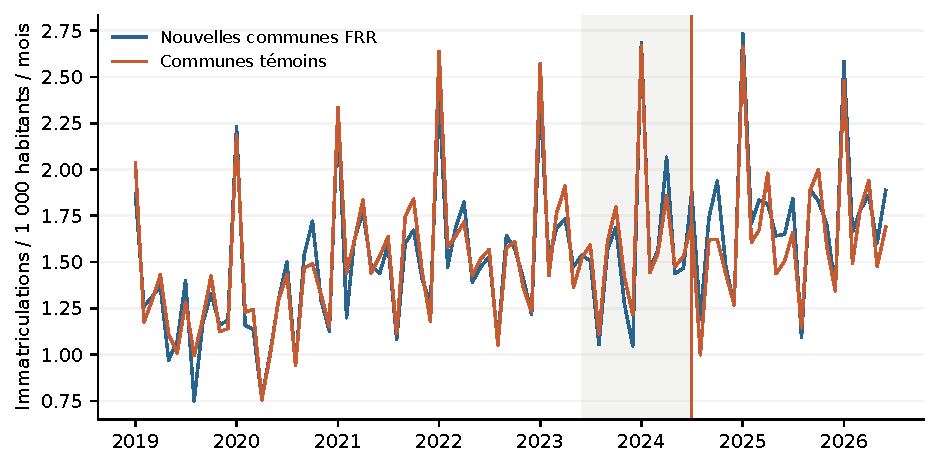
\includegraphics[width=\linewidth]{../results/figures/border_trends.pdf}\caption{Niveaux dans les paires frontalières}\notes{Deux séries exprimées par mille habitants, avec une population de référence fixe. Zone grise : de l’annonce à juin 2024. La hausse dans les témoins n’exclut pas un effet indirect plus faible que leur tendance contrefactuelle.}\end{figure}
\begin{figure}[htbp]\centering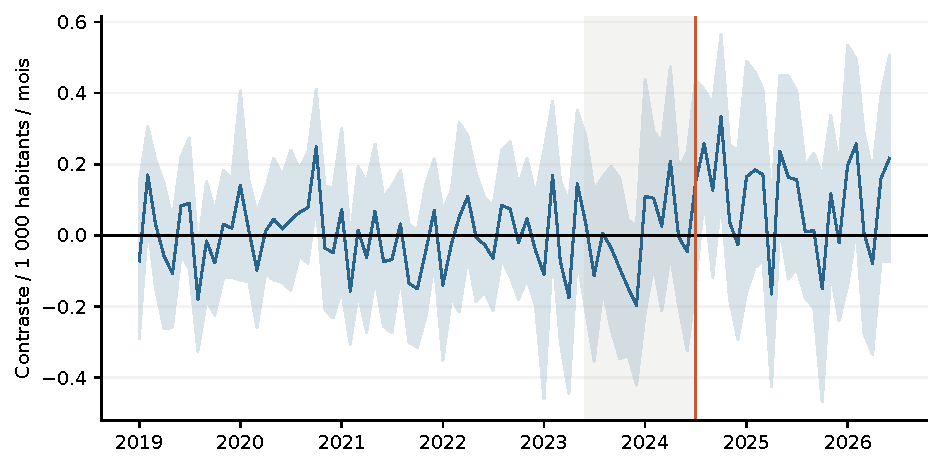
\includegraphics[width=\linewidth]{../results/figures/season_adjusted_event_study.pdf}\caption{Diagnostic après retrait de la saisonnalité propre aux paires}\notes{Chaque mois est comparé à la moyenne du même mois calendaire en 2019–2022, pour sa paire. Les restrictions préalables ont un rang de 41 et restent rejetées. Ce diagnostic ajouté après lecture des résultats ne remplace pas la normalisation principale.}\end{figure}

La référence moyenne principale ne contient ni la période d’annonce 2023–2024 ni les mois de premier traitement. Les fausses réformes 2021 et 2022 utilisent des observations sans annonce FRR. Juillet 2023 est conservé comme période d’annonce, jamais comme placebo sans annonce de politique. Le changement de base à 2019, la pondération en population et l’exclusion des futures FRR+ sont rapportés sans sélectionner les résultats favorables. Les résultats obtenus en excluant successivement les paires dont la commune traitée appartient à un département donné sont disponibles dans \texttt{leave\_one\_department\_out.csv}. Le département du témoin n’est pas le critère de cette exclusion.

Une analyse de sensibilité ajoutée après l’examen des résultats ajuste, sur janvier 2019–mai 2023, une tendance linéaire propre à chaque paire et des termes calendaires puis extrapole au second semestre 2024. Le résultat est enregistré dans \texttt{linear\_trend\_sensitivity.csv}. Cette extrapolation impose une évolution linéaire pendant et après des chocs macroéconomiques ; elle ne fournit pas de preuve que cette restriction soit vraie. Un résultat positif ne suffit donc pas à rétablir la validité du modèle causal.

Le modèle de comptage conditionne la vraisemblance de Poisson sur les totaux paire–mois, ce qui élimine les paramètres paire–temps. Le partage traité/témoin conserve un intercept estimé pour chaque paire : tous les effets fixes ne sont donc pas éliminés par conditionnement. Comme l’indicateur de période postérieure est identique dans les mois d’une période, les dénombrements des côtés traité et témoin peuvent être additionnés séparément sur les deux périodes pour estimer le coefficient et ce paramètre de nuisance. L’exponentielle du coefficient est le changement du rapport des taux des côtés traité et témoin, sous le modèle, et non un effet sur le total. Les paramètres non linéaires et les petits totaux informatifs peuvent induire un biais de taille finie ; aucune correction n’est réalisée ici. Les paires dans lesquelles un côté ne présente jamais d’immatriculation sont séparées ; celles dont le total est nul ne sont pas informatives. Leur exclusion et les pondérations expliquent pourquoi le rapport de taux ne se lit pas comme le contraste par habitant divisé par une seule moyenne préalable.

\section{Maintien administratif des cohortes}
\begin{table}[htbp]\centering\small\caption{Maintien administratif : cohortes des communes frontalières}\begin{tabularx}{\linewidth}{Xrrr}
\toprule
Horizon / groupe / cohorte & Suivies & Inconnues & Actives (\%) \\
\midrule
12 mois / FRR / 2019–22 & 27\,916 & 1 & 89,9 \\
12 mois / FRR / 2024 & 7\,980 & 0 & 89,0 \\
12 mois / témoin / 2019–22 & 33\,734 & 0 & 89,7 \\
12 mois / témoin / 2024 & 9\,298 & 0 & 89,0 \\
18 mois / FRR / 2019–22 & 27\,916 & 1 & 85,4 \\
18 mois / FRR / 2024 & 7\,980 & 0 & 84,3 \\
18 mois / témoin / 2019–22 & 33\,734 & 0 & 85,5 \\
18 mois / témoin / 2024 & 9\,298 & 0 & 84,0 \\
\bottomrule
\end{tabularx}
\notes{État A à l’anniversaire ; taux calculé parmi les états connus. 2019–22 : cohortes de juillet–décembre agrégées sur quatre années. 2024 : juillet–décembre. Taux pondérés par le nombre d’entrants, et non moyennes des taux communaux. La comparaison ne mesure pas un effet causal sur la survie.}\end{table}

Les cohortes éligibles au suivi atteignent l’anniversaire au plus tard le 30 juin 2026. Les états inconnus restent dans un dénominateur distinct ; les bornes inférieures et supérieures et les cohortes censurées sont dans le Parquet agrégé. L’état A à un anniversaire peut suivre une fermeture et une réouverture. Il ne renseigne pas sur la production ou la continuité de l’exploitation. Les créations sous une nouvelle politique peuvent avoir une composition différente ; il serait incorrect d’interpréter leur taux comme le résultat d’un traitement assigné aléatoirement aux entrants.

\section{Vérifications indépendantes internes}
Le contrôle institutionnel a vérifié les textes historiques, la distinction entre la liste et les droits, les anciennes ZRR et les décisions locales requises. Il a refait la topologie des \BorderPairs{} paires à partir des géométries officielles. Le contrôle économétrique a recalculé le contraste de différences, la vraisemblance conditionnelle et le test bootstrap par une implémentation distincte ; il a aussi identifié les échecs de tendances préalables et la dépendance des rôles administratifs.

L’audit de données a sélectionné vingt cellules commune–mois, avec une graine enregistrée et une stratification selon le traitement, la période et des dénombrements nuls ou positifs. Il a réextrait les fichiers bruts officiels, les périodes historiques et les successions, puis confronté 340 dénombrements aux cellules finales. Vingt établissements anonymisés dans le rapport ont également fait l’objet de 180 vérifications d’attributs. Aucun écart n’a été détecté dans ces contrôles. Le panel équilibré et les identités de décomposition ont été vérifiés globalement. Ce succès de reconstruction ne signifie pas que toute erreur dans le registre ou toute sélection institutionnelle serait absente.

La vérification de langue est réalisée par un agent d’IA distinct ; elle n’est pas présentée comme une relecture par une personne de langue maternelle française. Les rapports A–D sont des contrôles internes, sans statut de revue académique extérieure. Ils vérifient des faits, des calculs, la cohérence du texte et la portée déclarée des conclusions. Leurs résultats ne transforment pas les comparaisons ou les discontinuités en effets causaux.

\section{Journal des décisions et disponibilité}
Les documents \texttt{design\_before\_results.md} et \texttt{design\_changes.md} distinguent les choix arrêtés avant les résultats de ceux introduits ensuite. L’arrêt de la fenêtre en décembre 2024 a été décidé avant l’estimation, après la découverte de l’effet rétroactif de FRR+. Les diagnostics de saisonnalité, la structure conjointe intégrant les bassins et l’analyse exploratoire de densité sont consignés avec leur calendrier. Aucune modification n’est présentée comme un pré-enregistrement externe.

Le manuscrit est compilable à partir des tables et figures générées. Les données individuelles intermédiaires restent locales. Les agrégats diffusés, leurs conditions de réutilisation et les sources exclues de la redistribution sont définis dans le dossier de réplication. Les empreintes distinguent les versions locales de la publication éventuelle en archive ouverte ; cette dernière est séparée d’une publication dans une revue à comité de lecture.
\end{document}
